\section{Autonomous Walking}
\label{sec::54_aw}
\subsection{Data Acquisition}
\label{sec::541_da}
\begin{figure}[h]
	\centering
	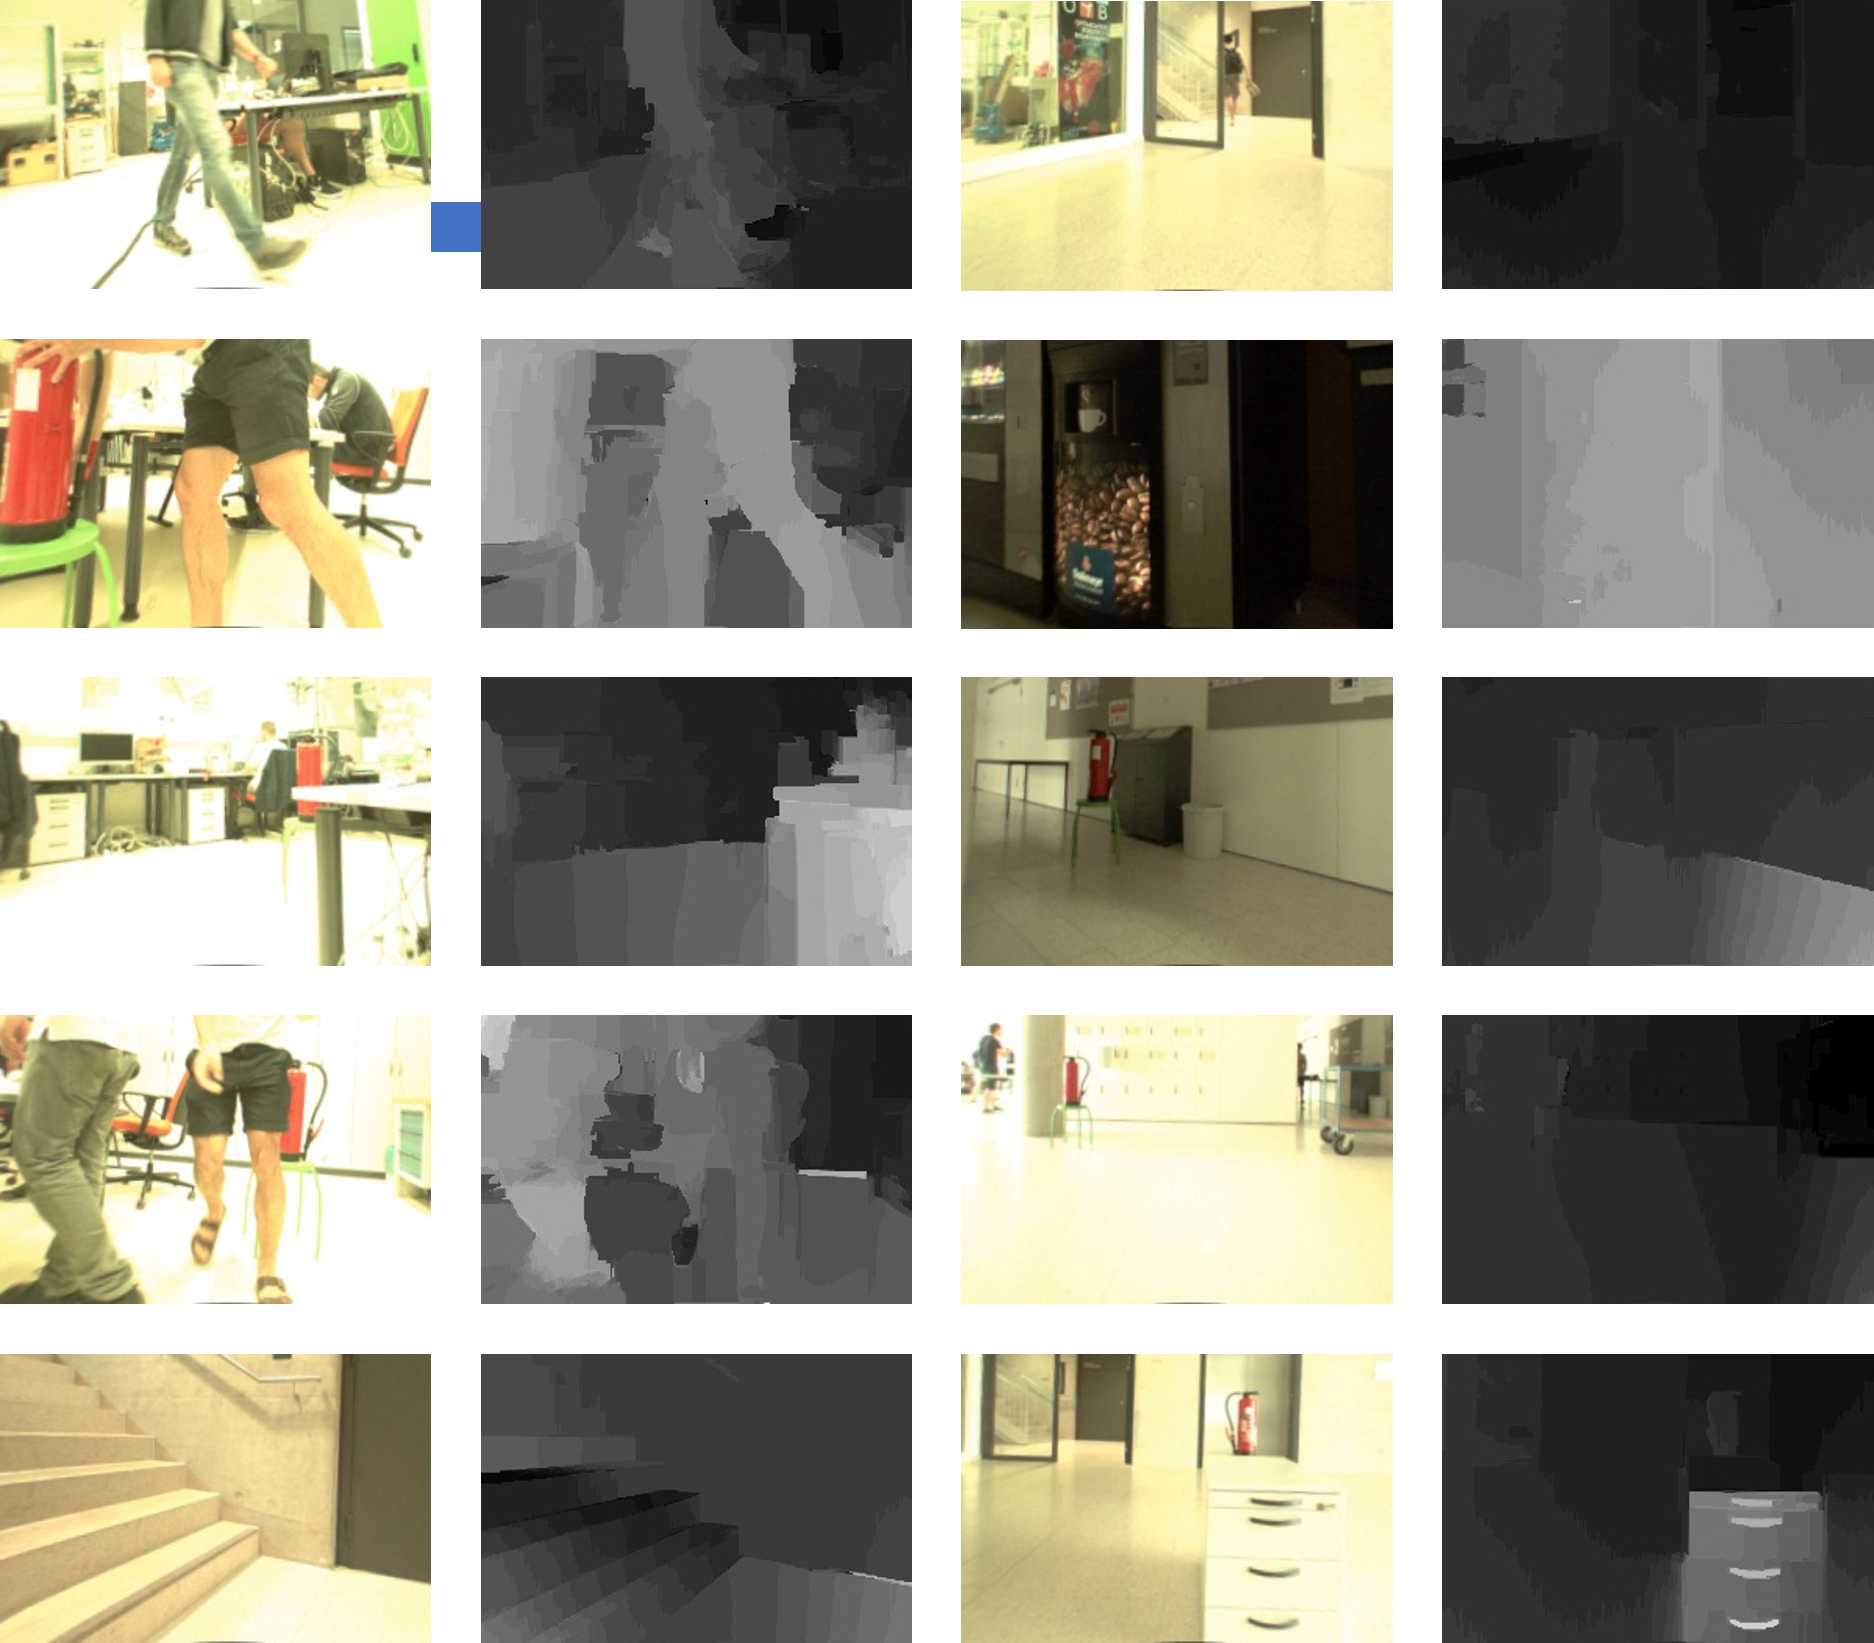
\includegraphics[scale=.4]{chapters/05_experiments/04_autonomous_walking/dataset_diversity.png}
	\caption{}
	\label{fig::542_dataset}
\end{figure}
\subsection{Network Architecture and Training}
\begin{figure}[h]
	\centering
	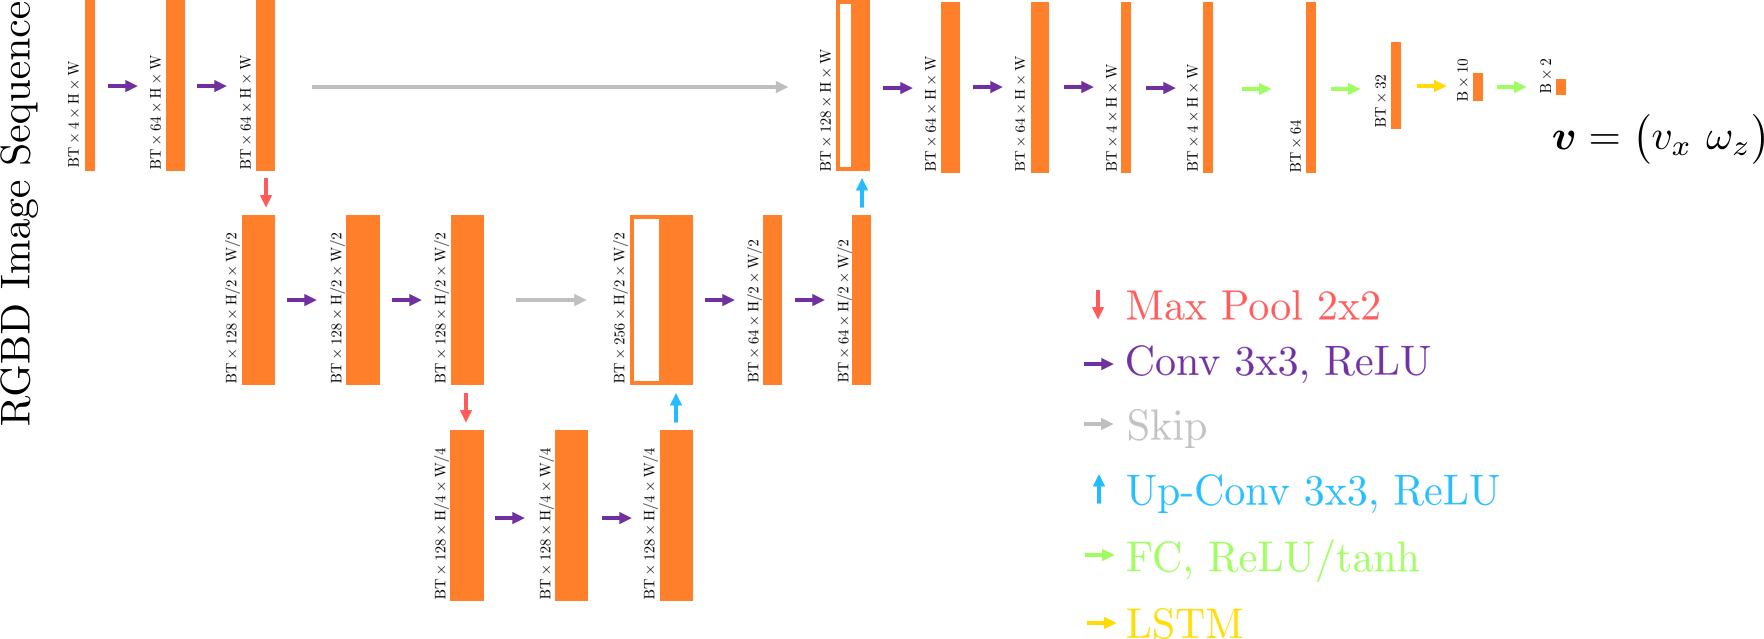
\includegraphics[scale=.5]{chapters/05_experiments/04_autonomous_walking/unet.png}
	\caption{}
	\label{fig::542_unet}
\end{figure}
\begin{figure}[h]
	\centering
	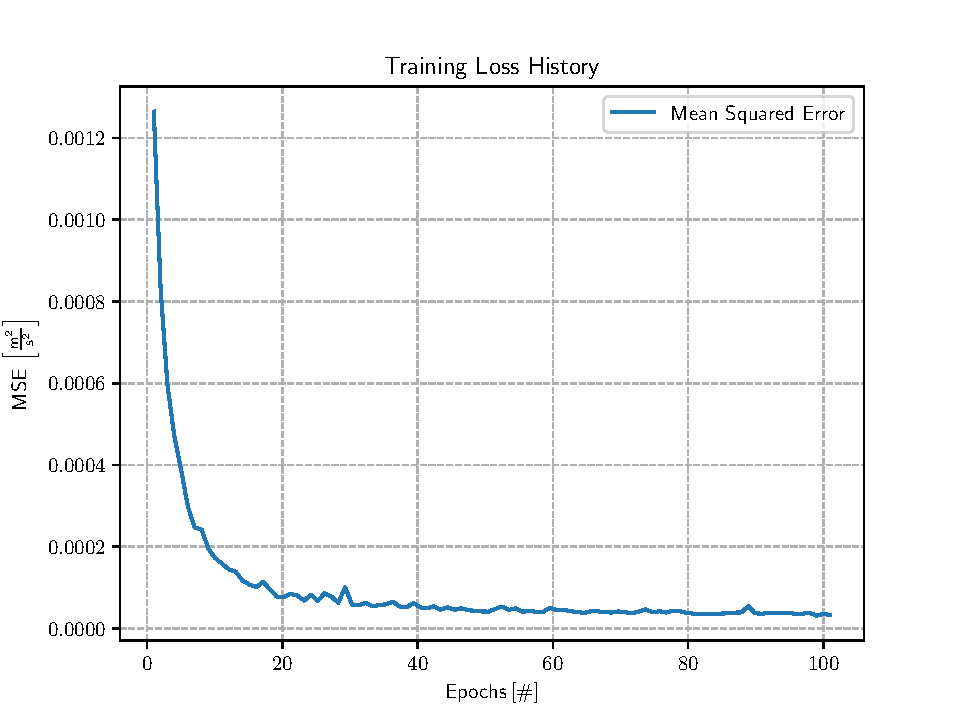
\includegraphics[scale=.6]{chapters/05_experiments/04_autonomous_walking/05_07_19_loss_history.pdf}
	\caption{}
	\label{fig::542_loss}
\end{figure}
\begin{figure}[h]
	\centering
	\subcaptionbox{}%
	[.4\linewidth]{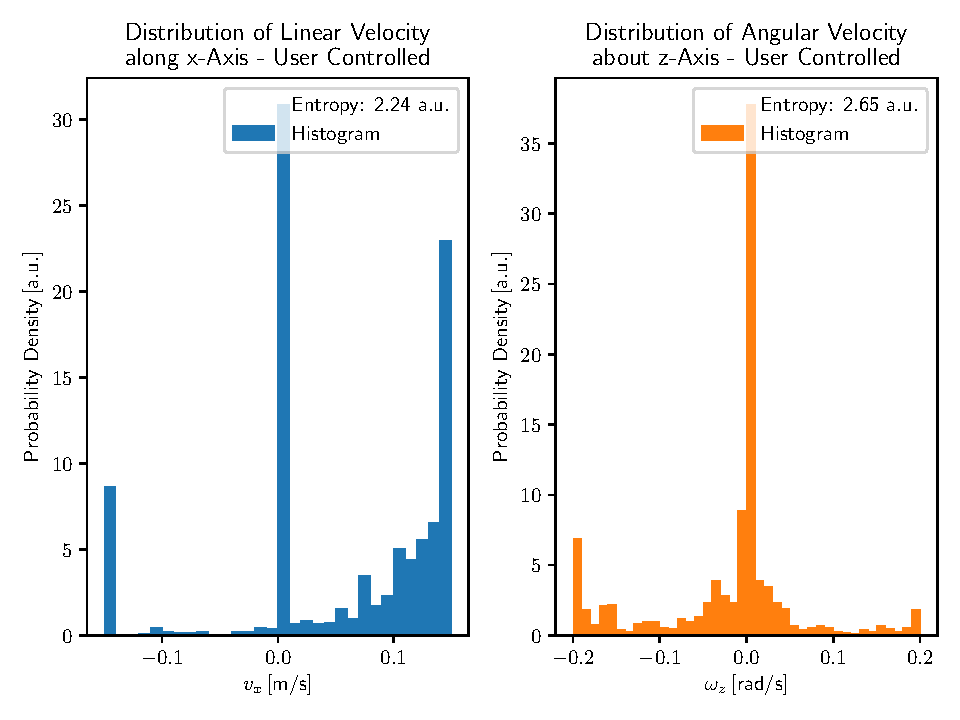
\includegraphics[scale=.35]{chapters/05_experiments/04_autonomous_walking/user_entropy.pdf}}
	\subcaptionbox{}%
	[.4\linewidth]{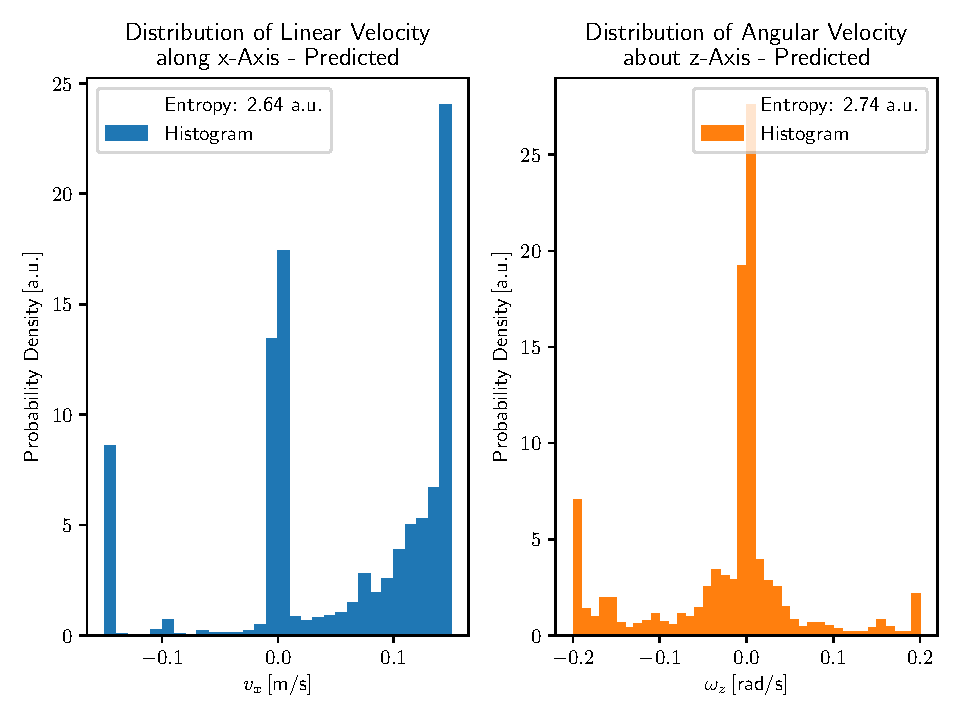
\includegraphics[scale=.35]{chapters/05_experiments/04_autonomous_walking/predicted_entropy_kldivx_0_33_kldivz_0_06_imgs_13441_duration_4_ms.pdf}}
	\caption{KL divergence x 0.33, KL divergence z 0.06, validation split on 13441 imgs, average duration 4 ms}
	\label{fig::542_training_dist}
\end{figure}
% compute kl divergence for whole set -> argue that this holds true for all 
\subsection{Performance in Test Environment}
\begin{figure}[h]
	\centering
	\subcaptionbox{Straight Walk}%
	[.4\linewidth]{\animategraphics[height=1.2in,loop,autoplay]{20}{chapters/05_experiments/04_autonomous_walking/straight_walk_01/frame-}{001}{033}}
	\subcaptionbox{Curved Walk}%
	[.4\linewidth]{\animategraphics[height=1.2in,loop,autoplay]{20}{chapters/05_experiments/04_autonomous_walking/curved_walk_02/frame-}{001}{039}}
	\subcaptionbox{Obstacle Avoidance}%
	[.4\linewidth]{\animategraphics[height=1.2in,loop,autoplay]{20}{chapters/05_experiments/04_autonomous_walking/obstacle_walk_02/frame-}{001}{017}}
	\subcaptionbox{Environment Scanning}%
	[.4\linewidth]{\animategraphics[height=1.2in,loop,autoplay]{20}{chapters/05_experiments/04_autonomous_walking/out_of_sight_walk_01/frame-}{001}{075}}
	\caption{}
	\label{fig::53_aw_gif_basic}
\end{figure} 
\begin{figure}[h]
	\centering
	\subcaptionbox{Straight Walk - Dynamic Balance}%
	[.4\linewidth]{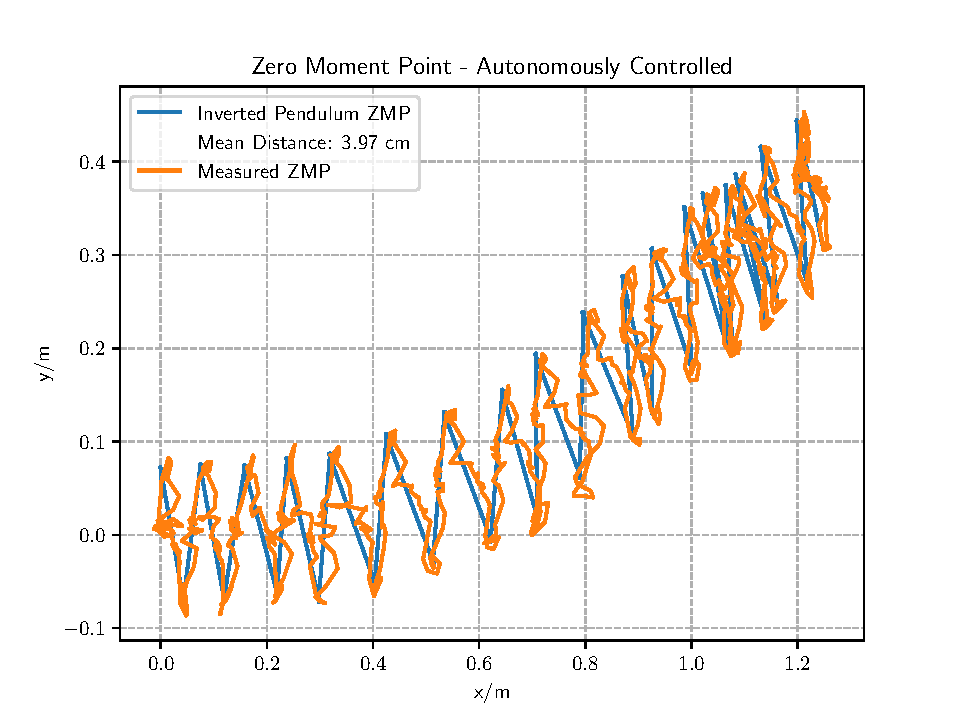
\includegraphics[scale=.35]{chapters/05_experiments/04_autonomous_walking/straight_walk_01_zmp.pdf}}
	\subcaptionbox{Straight Walk - Behavior}%
	[.4\linewidth]{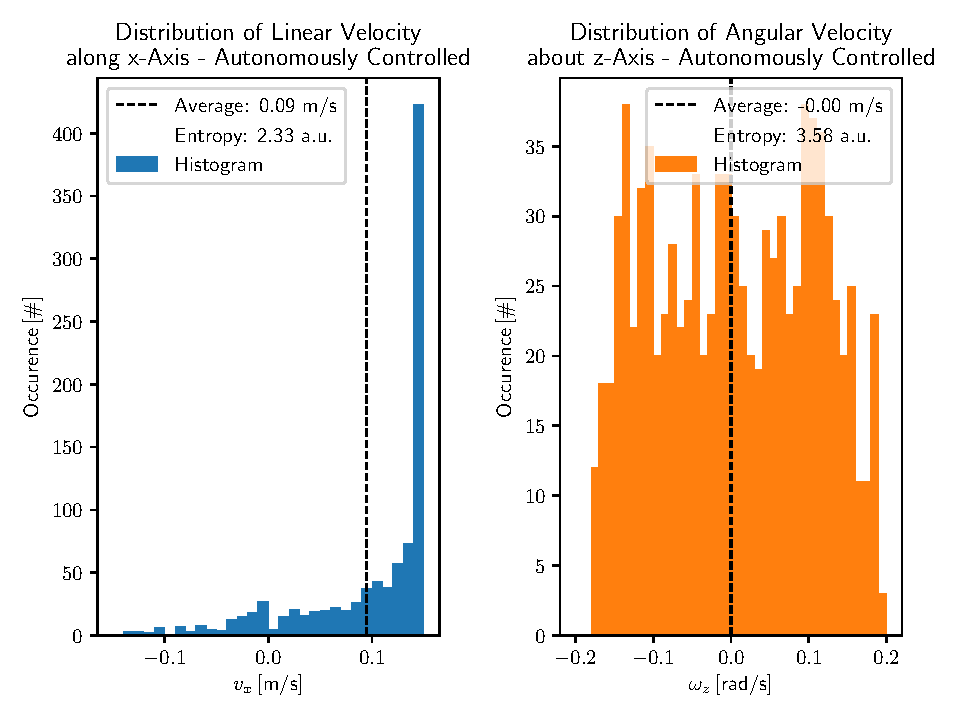
\includegraphics[scale=.35]{chapters/05_experiments/04_autonomous_walking/straight_walk_01_entropy.pdf}}
	\subcaptionbox{Curved Walk - Dynamic Balance}%
	[.4\linewidth]{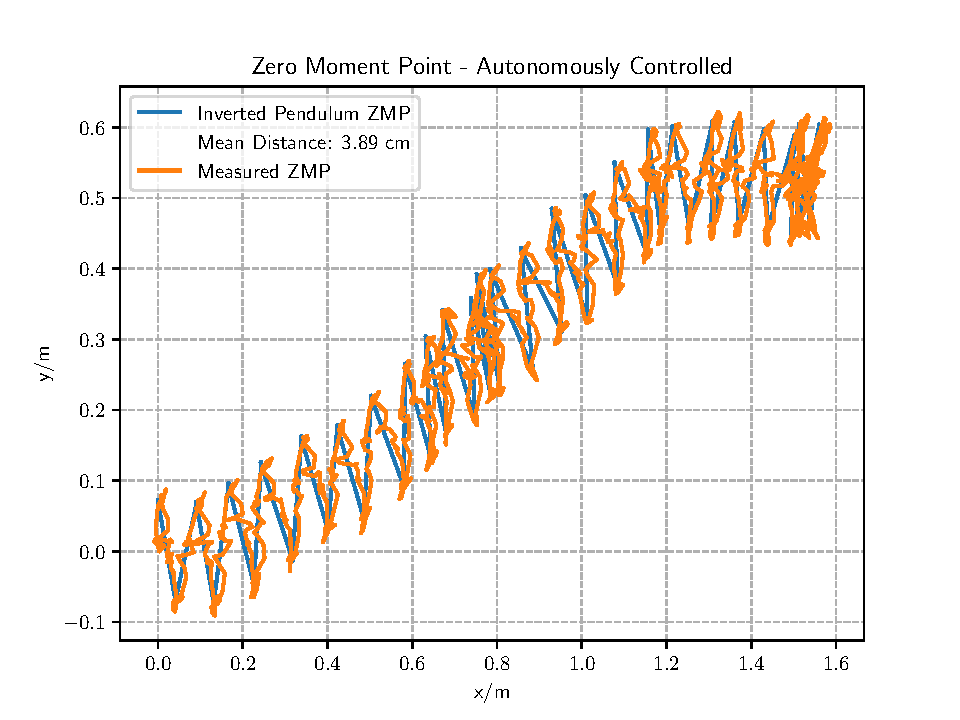
\includegraphics[scale=.35]{chapters/05_experiments/04_autonomous_walking/curved_walk_01_zmp.pdf}}
	\subcaptionbox{Curved Walk - Behavior}%
	[.4\linewidth]{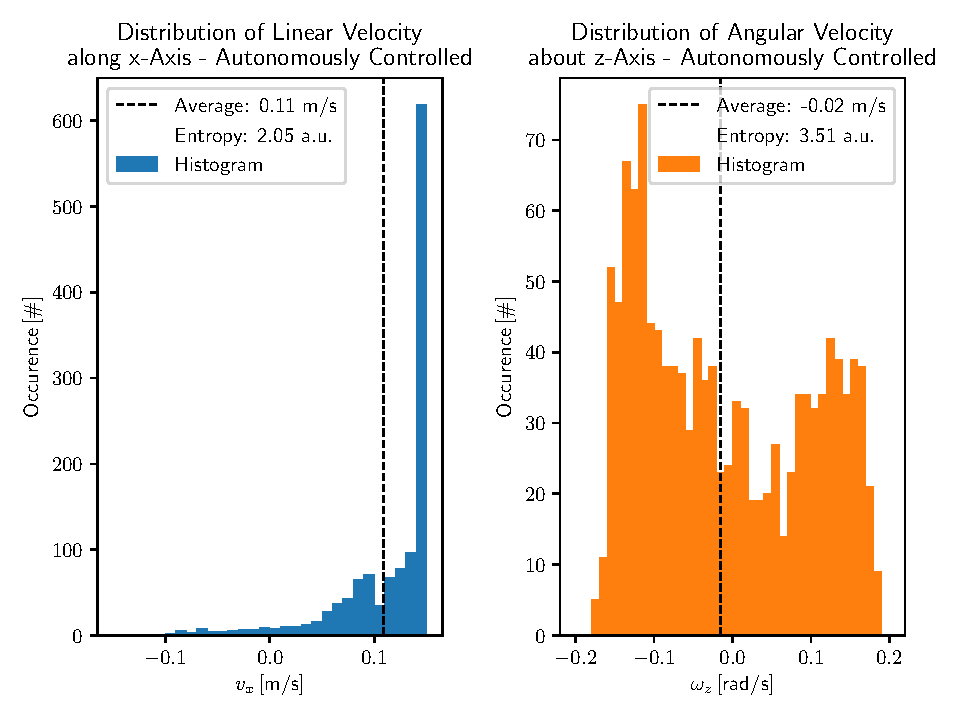
\includegraphics[scale=.35]{chapters/05_experiments/04_autonomous_walking/curved_walk_01_entropy.pdf}}
	\subcaptionbox{Obstacle Avoidance - Dynamic Balance}%
	[.4\linewidth]{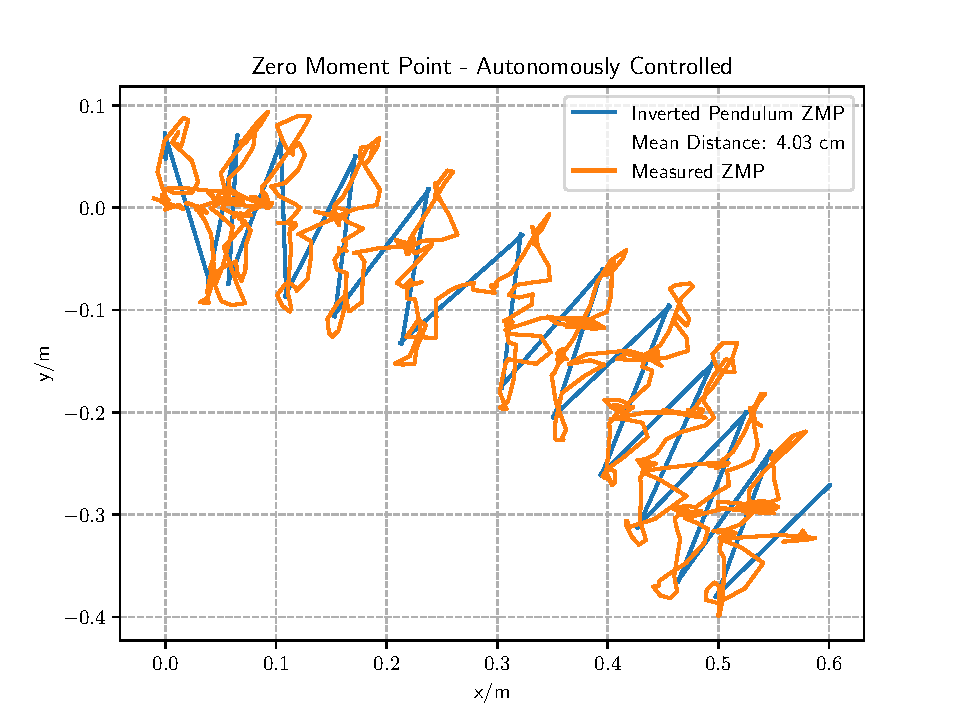
\includegraphics[scale=.35]{chapters/05_experiments/04_autonomous_walking/obstacle_walk_02_zmp.pdf}}
	\subcaptionbox{Obstacle Avoidance - Behavior}%
	[.4\linewidth]{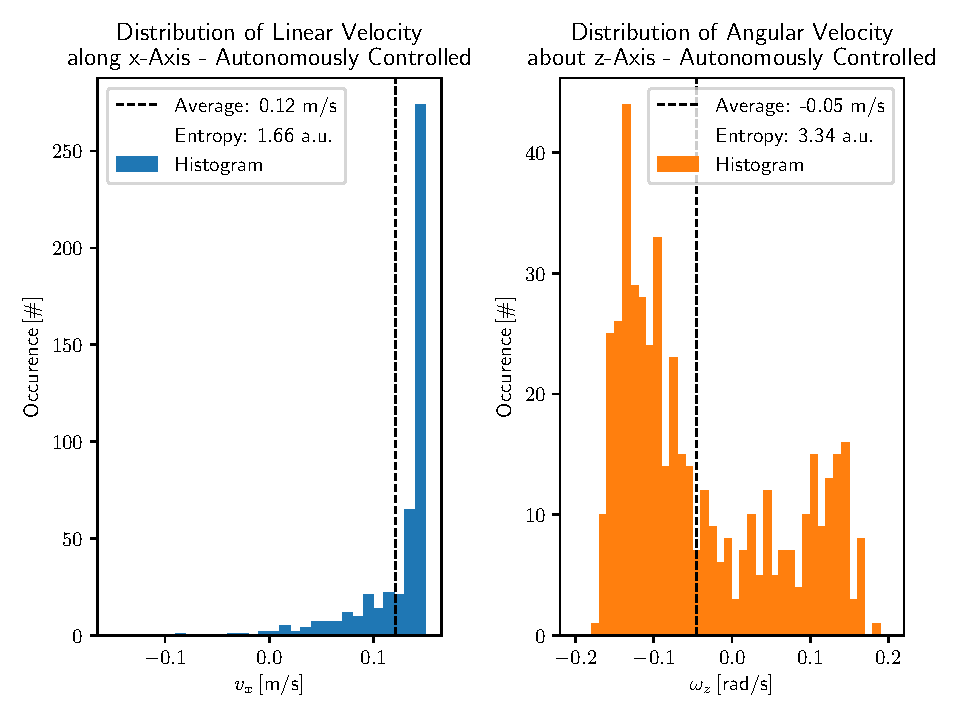
\includegraphics[scale=.35]{chapters/05_experiments/04_autonomous_walking/obstacle_walk_02_entropy.pdf}}
	\subcaptionbox{Environment Scanning - Dynamic Balance}%
	[.4\linewidth]{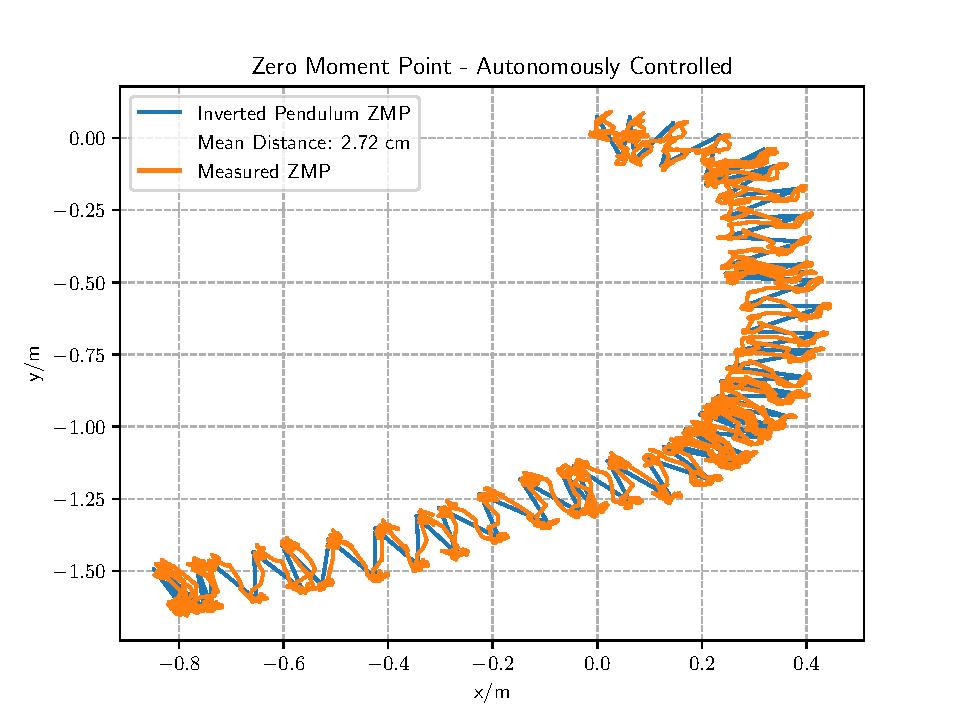
\includegraphics[scale=.35]{chapters/05_experiments/04_autonomous_walking/out_of_sight_walk_01_zmp.pdf}}
	\subcaptionbox{Environment Scanning - Behavior}%
	[.4\linewidth]{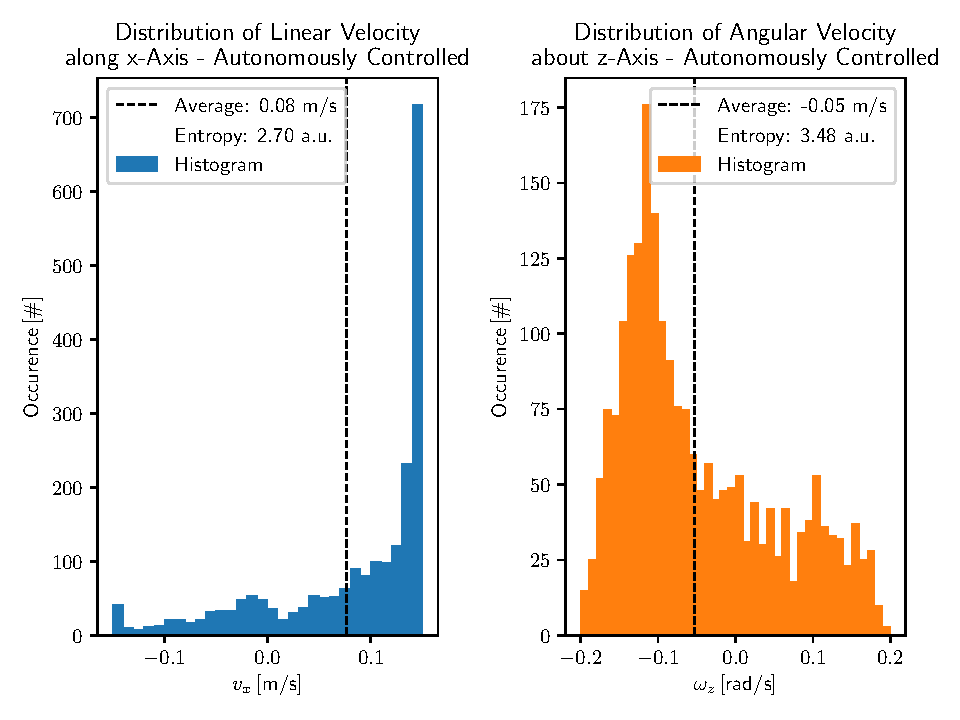
\includegraphics[scale=.35]{chapters/05_experiments/04_autonomous_walking/out_of_sight_walk_01_entropy.pdf}}
	\caption{}
	\label{fig::53_aw_basic}
\end{figure} 
\begin{figure}[h]
	\centering
	\subcaptionbox{Dynamic Environment}%
	[.4\linewidth]{\animategraphics[height=1.2in,loop,autoplay]{20}{chapters/05_experiments/04_autonomous_walking/dynamic_walk_01/frame-}{001}{031}}
	\subcaptionbox{Semantic Understanding}%
	[.4\linewidth]{\animategraphics[height=1.2in,loop,autoplay]{20}{chapters/05_experiments/04_autonomous_walking/semantic_walk_01/frame-}{001}{046}}
	\caption{}
\label{fig::53_aw_gif_additional}
\end{figure} 
\begin{figure}[h]
	\centering
	\subcaptionbox{Dynamic Environment - Dynamic Balance}%
	[.4\linewidth]{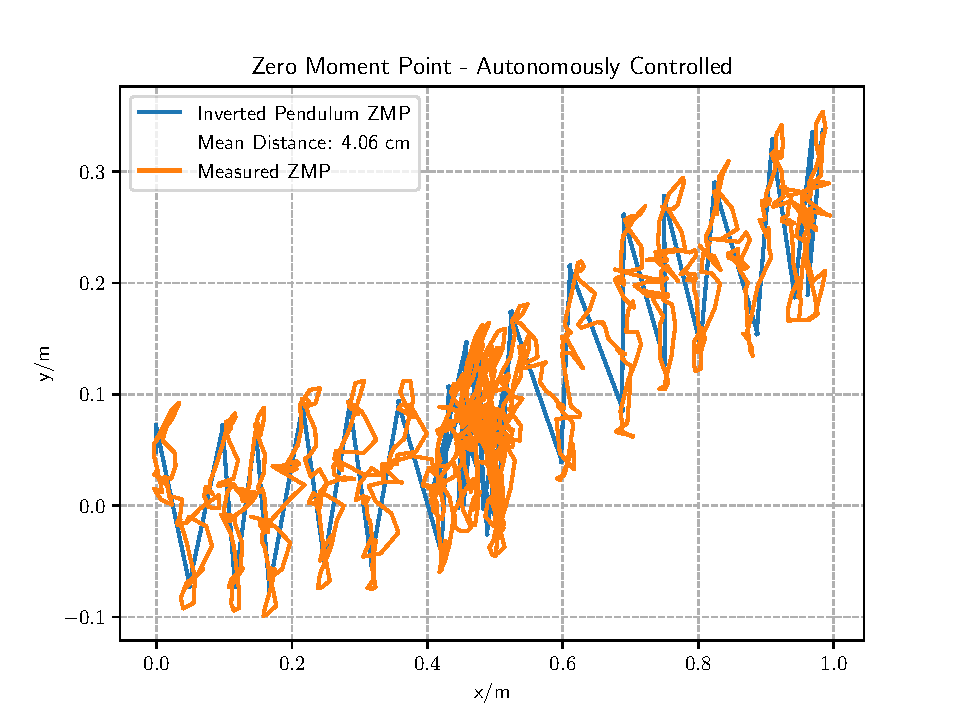
\includegraphics[scale=.35]{chapters/05_experiments/04_autonomous_walking/dynamic_walk_01_zmp.pdf}}
	\subcaptionbox{Dynamic Environment - Behavior}%
	[.4\linewidth]{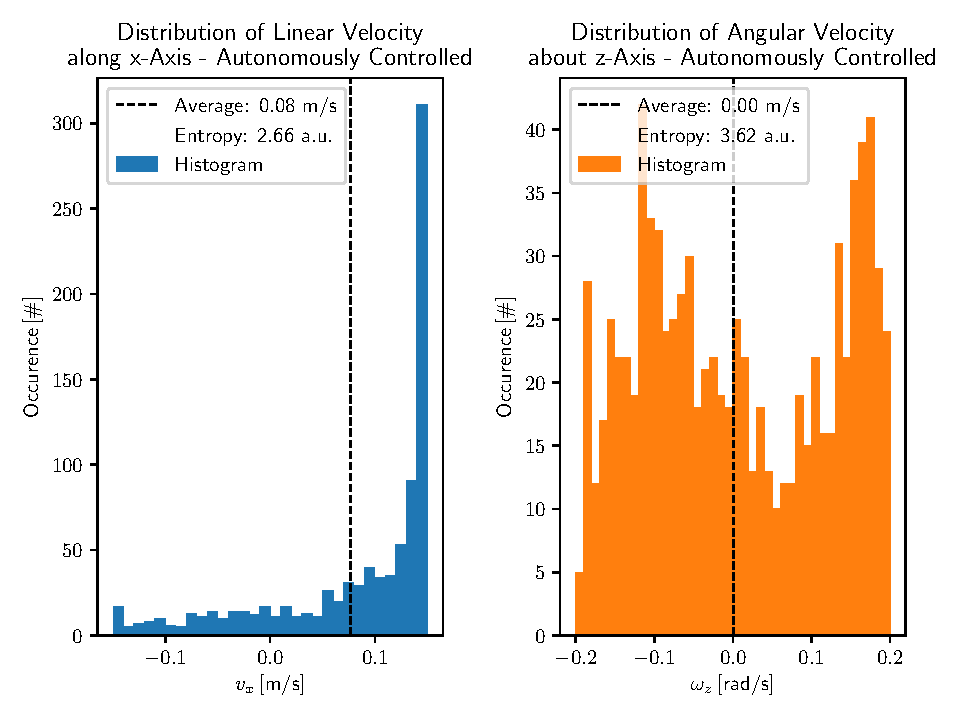
\includegraphics[scale=.35]{chapters/05_experiments/04_autonomous_walking/dynamic_walk_01_entropy.pdf}}
	\subcaptionbox{Semantic Understanding - Dynamic Balance}%
	[.4\linewidth]{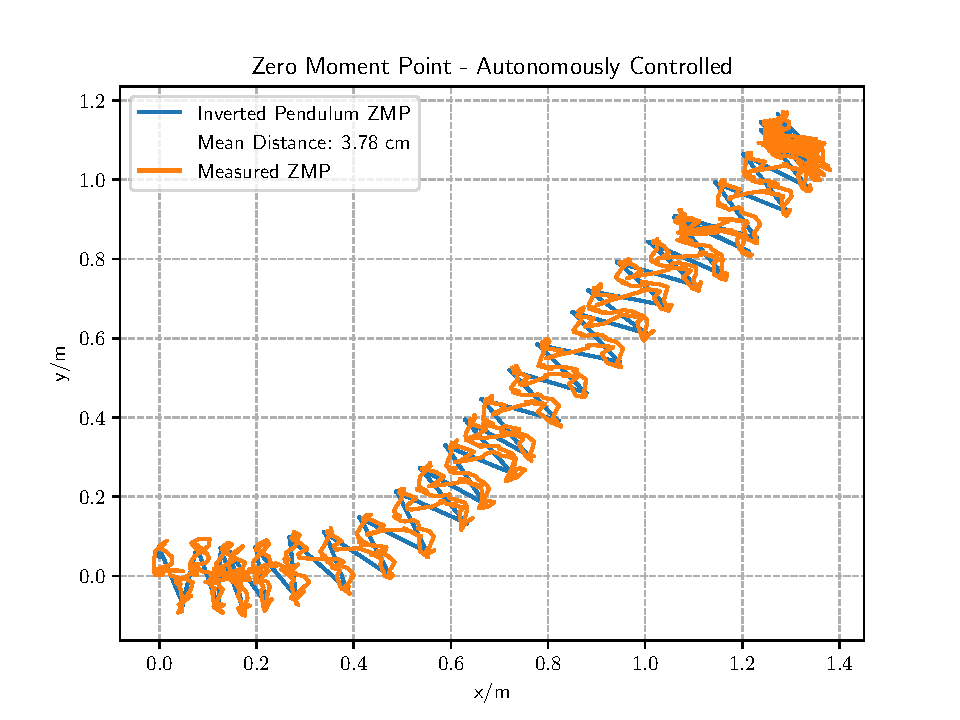
\includegraphics[scale=.35]{chapters/05_experiments/04_autonomous_walking/semantic_walk_01_zmp.pdf}}
	\subcaptionbox{Semantic Understanding - Behavior}%
	[.4\linewidth]{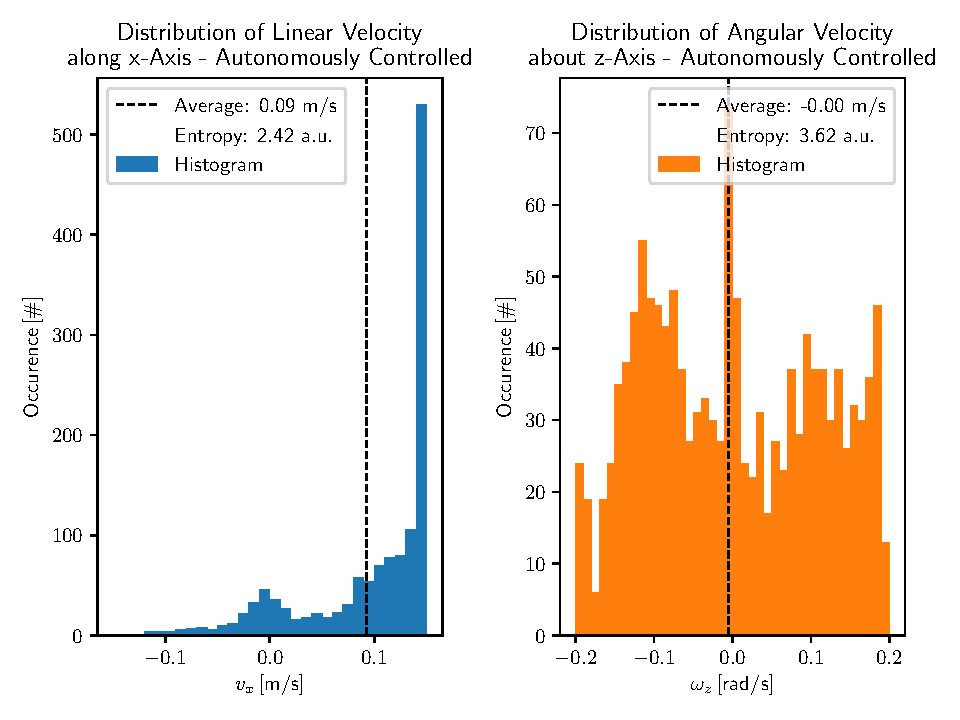
\includegraphics[scale=.35]{chapters/05_experiments/04_autonomous_walking/semantic_walk_01_entropy.pdf}}
	\caption{}
	\label{fig::53_aw_additional}
\end{figure}
\begin{figure}[h]
	\centering
	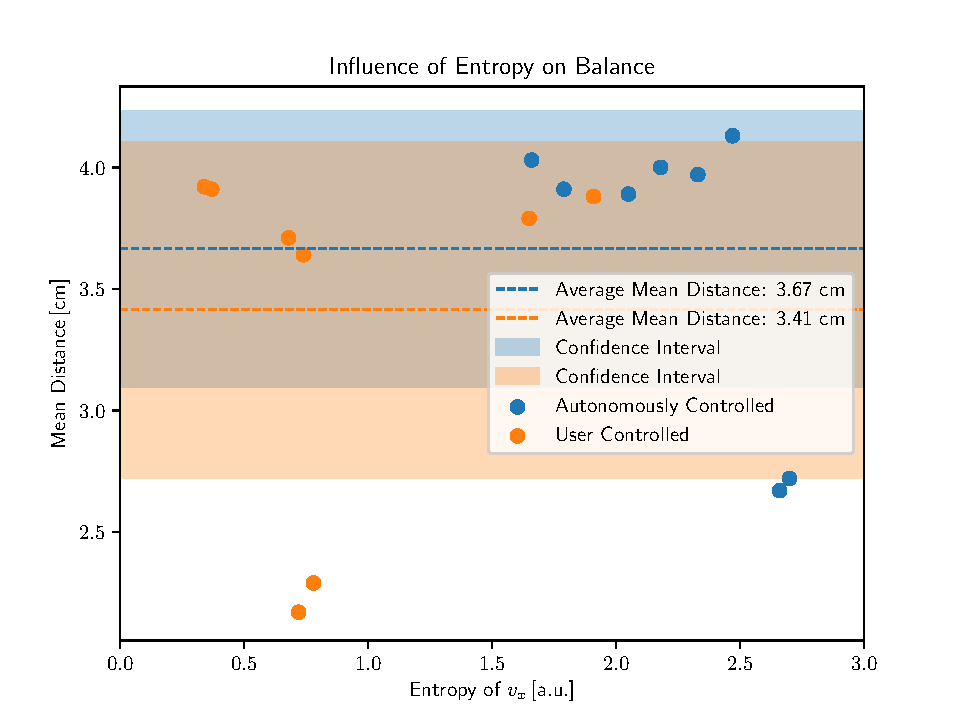
\includegraphics[scale=.6]{chapters/05_experiments/04_autonomous_walking/entropy_against_balance.pdf}
	\caption{meanaw 3.67, meanuc 3.41, stdaw 0.56, stduc 0.69}
	\label{fig::542_entropy_balance}
\end{figure}
\subsection{Proximal Policy Optimization}
